\documentclass[
    landscape,      % landscape or portrait
    paperwidth = 1200mm,
    paperheight = 900mm,
    fontscale = 0.4,
    margin = 1.7cm,
]{baposter}
\definecolor{lightblue}{rgb}{0.145,0.6666,1}
\usepackage{times}
\usepackage{tikz}
\usepackage{floatrow}
\usepackage{hyperref}
%
% these are some of my own latex definitions
%

\newcommand{\lzhu}{\underline{L.~Zhu}}
\renewcommand{\topfraction}{.75}

%%%% for manuscript submission
%\newenvironment{annotation}{\bfseries}{\normalfont}
\newenvironment{annotation}{\color{red}}{\color{black}}
%\newcommand{\clearemptydoublepage}{\newpage{\pagestyle{empty}\cleardoublepage}}

%%% for inserting figures
\newcommand{\putfigure}[2]{%
  \begin{center}
%    \epsfig{file=#2,width=#1}
     \includegraphics[width=#1]{#2}%
  \end{center}
}

% two figs left and right aligned at the bottom
\newcommand{\putfigureLR}[4]{%
  \begin{center}
     \begin{tabular}{cc}
     \includegraphics[width=#1]{#2} &
     \includegraphics[width=#3]{#4}
     \end{tabular}
  \end{center}
}

% two figs left and right aligned at the bottom
\newcommand{\putfigurecaptionLR}[6]{%
    \hspace{2em}
    \begin{minipage}{#1}
    %\centering
    \footnotesize
    \textbf{#2}
    \itshape
    #3
    \end{minipage}
    \hspace{1em}
    \begin{minipage}{#4}
    % \centering
    \footnotesize
    \textbf{#5}
    \itshape
    #6
    \end{minipage}

}


% four figs left and right
\newcommand{\putfigureLRLR}[5]{%
  \begin{center}
     \begin{tabular}{cc}
     \includegraphics[width=#1]{#2} &
     \includegraphics[width=#1]{#3} \\
     \includegraphics[width=#1]{#4} &
     \includegraphics[width=#1]{#5}
     \end{tabular}
  \end{center}
}

% two figs left and right aligned at the top
\def\imagetop#1{\vtop{\null\hbox{#1}}}
\newcommand{\putfigureLRt}[4]{%
  \begin{center}
     \begin{tabular}{cc}
     \imagetop{\includegraphics[width=#1]{#2}} &
     \imagetop{\includegraphics[width=#3]{#4}}
     \end{tabular}
  \end{center}
}

% three figs in a row
\newcommand{\putfigureLCR}[6]{%
  \begin{center}
     \begin{tabular}{ccc}
     \includegraphics[width=#1]{#2} &
     \includegraphics[width=#3]{#4} &
     \includegraphics[width=#5]{#6}
     \end{tabular}
  \end{center}
}

% three figs in a row aligned at the top
\newcommand{\putfigureLCRt}[6]{%
  \begin{center}
     \begin{tabular}{ccc}
     \imagetop{\includegraphics[width=#1]{#2}} &
     \imagetop{\includegraphics[width=#3]{#4}} &
     \imagetop{\includegraphics[width=#5]{#6}}
     \end{tabular}
  \end{center}
}

% one left and two in a column at right
\newcommand{\putfigureLRR}[5]{%
  \begin{center}
     \begin{tabular}{cc}
     \includegraphics[width=#1]{#2} &
     \parbox[b]{#3}{\includegraphics[width=#3]{#4}
     \includegraphics[width=#3]{#5}}
     \end{tabular}
  \end{center}
}

% two left in a column and one at right
\newcommand{\putfigureLLR}[5]{%
  \begin{center}
     \begin{tabular}{cc}
     \parbox[b]{#1}{\includegraphics[width=#1]{#2}\\
     \includegraphics[width=#1]{#3}} &
     \includegraphics[width=#4]{#5}
     \end{tabular}
  \end{center}
}

% one fig at left and text in the right
\newcommand{\putfigureL}[4]{%
  \begin{center}
  \parbox{#1}{\includegraphics[width=#1]{#2}}
  \parbox{#3}{#4}
  \end{center}
}

% two figs at left and text in the right
\newcommand{\putfigureLL}[5]{%
  \begin{center}
  \parbox{#1}{\includegraphics[width=#1]{#2}
              \includegraphics[width=#1]{#3}}
  \parbox{#4}{#5}
  \end{center}
}

% two columns of figs
\newcommand{\putfigureLLRR}[6]{%
  \begin{center}
  \parbox{#1}{\includegraphics[width=#1]{#2}
              \includegraphics[width=#1]{#3}}
  \parbox{#4}{\includegraphics[width=#4]{#5}
              \includegraphics[width=#4]{#6}}
  \end{center}
}

%%% two columns texts
\newcommand{\twocol}[4]{%
  \begin{center}
  \parbox[t][][t]{#1}{#2}
  \parbox[t][][t]{#3}{#4}
  \end{center}
}

%%% slide heading
\newcommand{\slideheading}[1]{%
  \begin{center}
    \large\bf
    \shadowbox{#1}%
  \end{center}
  \vspace{1ex minus 1ex}}

%%% some often used units
\newcommand{\kms}{km/s}
\renewcommand{\deg}{$^\circ$}
\newcommand{\Cel}{{\deg}C}

%%% math symbols: e, d (derivative), i (imaginary), T (transpose)
\newcommand{\me}{\mathrm{e}}
\newcommand{\md}{\mathrm{d}}
\newcommand{\mi}{\mathrm{i}}
\newcommand{\mT}{\mathrm{T}}

%%% differential operator
\newcommand{\dif}[2]{\frac{\md #1}{\md #2}}
\newcommand{\ddif}[2]{\frac{\md^2 #1}{\md #2^2}}
\newcommand{\dd}[1]{#1^{\prime\prime}}
\newcommand{\ddd}[1]{#1^{\prime\prime\prime}}
\newcommand{\pdif}[2]{\frac{\partial #1}{\partial #2}}
\newcommand{\pdifc}[2]{{#1}_{,#2}}
\newcommand{\pddif}[2]{\frac{\partial^2 #1}{\partial #2^2}}
\newcommand{\pdddif}[3]{\frac{\partial^2 #1}{\partial #2\partial #3}}
\newcommand{\grad}{\nabla}
\newcommand{\rgrad}{\overrightarrow{\grad}}
\newcommand{\lgrad}{\overleftarrow{\grad}}
\renewcommand{\div}{\nabla\cdot}
\newcommand{\curl}{\grad \times}
\newcommand{\laplace}{\grad^2}
\newcommand{\sgn}{\operatorname{sgn}}

\providecommand{\conjg}[1]{#1^{*}}
\providecommand{\abs}[1]{\lvert#1\rvert}
\providecommand{\norm}[1]{\lVert#1\rVert}

%%%  vectors
\newcommand{\vct}[1]{\mathbf{#1}}
\newcommand{\uct}[1]{\hat{\mathrm{#1}}}

%%% matrices
\newcommand{\mtx}[1]{\mathbf{#1}}

%%% tensors
\newcommand{\tensor}[1]{\mathbf{#1}}

%%% isotopes
\newcommand{\isotope}[2]{{}^{#1}#2}

\def\cossin{\begin{pmatrix}\cos{n \theta}\\ \sin{n \theta}\end{pmatrix}}
\def\sincos{\begin{pmatrix}\sin{n \theta}\\ \cos{n \theta}\end{pmatrix}}

%\DeclareMathOperator\erf{erf}
%\DeclareMathOperator\erfc{erfc}
\endinput


\begin{document}

\begin{poster}{
    % poster environment options
    grid = false,            % true or false
    columns = 3,
    colspacing = 0.6em,
    bgColorOne = white,
    bgColorTwo = white,
    background = plain,     % plain, shade-lr, shade-tb, user, none
    eyecatcher = true,      % eye catcher on the left of the title page
    % posterbox environment options
    borderColor = blue,
    headerColorOne = black,
    headerColorTwo = lightblue,
    headerFontColor = white,
    textborder = roundedleft,   % none, bars, coils, triangles, rectangle
                                % rounded, faded, roundedsmall, roundedleft
                                % roundedright
    headerborder = closed,      % none, closed, open
    headershape = roundedright, % rectangle, small-rounded, roundedleft,
                                % roundedright, rounded
    headershade = shadelr,      % plain, shadelr, shadetb, shade-tb-inverse
    boxshade = none,            % plain, shade-lr, shade-tb, none
    headerfont = \Large\bf\textsc,
    linewidth = 0.1 em,}
{
\includegraphics[height=9em]{USTC_logo_blue.jpg}}
{\Huge{3D Crust and Uppermost Mantle Structure beneath Tian Shan Region from ambient noise and earthquake surface waves}}
{
    \vspace{0.3em}
    Xiao Xiao$^1$ (\textcolor{blue}{xiaox17@mail.ustc.edu.cn}),
    Lianxing Wen$^{2,1}$ \\
    \vspace{0.3em}
    1. Laboratory of Seismology and Physics of Earth's Interior, University of Science and Technology of China  \\
    2. Department of Geosciences, State University of New York at Stony Brook  \\
}
{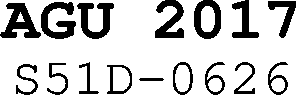
\includegraphics[height=5em]{2017_AGU_ID}}
\vspace{0.4cm}

\begin{posterbox}[column=0, row=0]{1. Introduction}
\setlength{\parskip}{3pt}
As a typical active intracontinental mountain range in Central Asia, Tian
Shan Mt serves as the prototype in studying geodynamic processes and mechanism
of intracontinental mountain building. In Tian Shan Mt. and nearby area,  There are three mainly geological blocks,
Tarim basin, Tian Shan Mountain and Junggar basin. To figure out underground structure and geological evolution history there,
We study 3D crust and the uppermost mantle structure beneath Tian Shan and close region
using ambient noise and earthquake surface waves.
\end{posterbox}

\begin{posterbox}[column=0, below=auto]{2. Data and Methods}
\setlength{\parskip}{3pt}
My data set contains 60 brand-band seismic stations mainly
locating at foot of Tian Shan mountain and joint area (Fig. 1.).
Several stations, situating at the sounthern foot of Altai Mt. and northern foot of Kunlun Mt.,
provide critical ray path coverage of Junggar amd Tarim basins.Our dataset includes vertical
component continuous record from 2015 to 2016 and teleseismic waveforms,
whose magnitudes are over 5.5, focal depths are shallower than 200 km and happened during
2013 and 2016.

We combine the group velocity dispersion curves measured from ambient noise and earthquake surface waves,
obtain lateral isotropic group velocity maps at different periods based on tomography and invert a 3D Vsv model of crust
and uppermost mantle down to about 70 km using a Monte Carlo Inversion method.



\begin{center}

\begin{minipage}{0.2\textwidth}
\footnotesize
\textbf{Fig. 1.}
\itshape
Map of research area. Red triangles represent broad-band seismic stations
in Tianshan area used in this study. Solid black thick lines show the faults.
The insert (top left) depicts telsesimic distribution. Red circles represent
epicenter of teleseismic used in this study, which happened from 2013 to 2016.
Dashed red square is study area. Two triangles represent two stations named as
AKS and KOL, which are in common line with this star-labelled earthquake.
\end{minipage}
\begin{minipage}{0.75\textwidth}
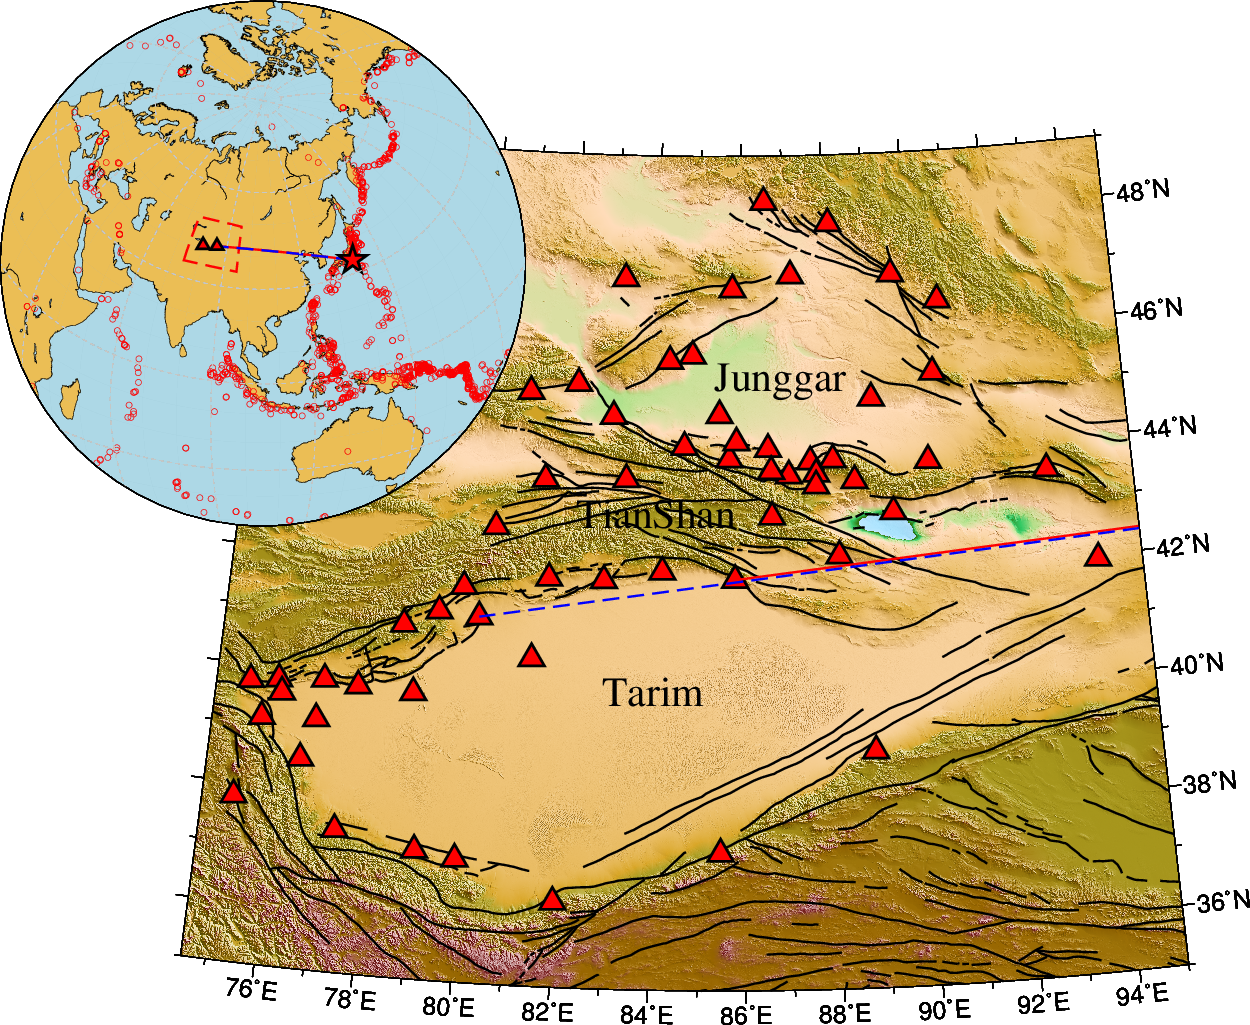
\includegraphics[width=\textwidth]{XJ}
\end{minipage}
\hspace{0.1cm}

\end{center}



We control quality of dispersion curves with spectral signal-noise-ratio (SNR) and standard deviation of measuremens.
For EGFs, we define signal-noise-ratio (SNR) as ratio of peak in signal window of surface
wave and root mean standard (rms) in noise window at each period and we measure dispersion curves every trimesters
which provides standard deviation of dispersion curve between a pair of station.
We measure dispersion curves from telesemic waveforms of different events of two stations.
These curves give final dispersion curve to be meadian of them and standard deviation at each periods (Fig. 2.).

We take weighted average of reliable dispersion curves measured from EGF and teleseismic waveform to be final
usable dispersion curves (Fig. 3.) and the weight is inverse of their standard deviation.



\putfigureLR{0.45\textwidth}{Pathnum}{0.45\textwidth}{JointDisp}

\hspace{0.1cm}

\putfigurecaptionLR{0.45\textwidth}
{Fig. 3.}
{Variation of dispersion curve numbers used for tomography due to dispersion curves quality control.The Dashed limegreen line and corresponding limegreen area shows number of used dispersion
curves measured from teleseismic with two-station method while Dashed red line and area denote number of those measured from EGF at each period. The
solid blue line indicates numbers of all used dispersion curves which are summation of above two.}
{0.45\textwidth}{Fig. 2.}
{Demos of combination of group velocity dispersion curves between two stations, AKS and KOL.
Red circles denote dispersion points measured from EGF while blue circles represent those measured from teleseismic.
Limegreen squares give combined dispersion curve. At overlap periods, green squares are weight average of blue and red circles
, in which weights are inverse of their error which summation of their errors gives error of combined dispersion curve.
}



\end{posterbox}

\begin{posterbox}[column=1]{3. 2D Group velocity Maps}

With combined dispersion curves, we use traditional surface wave tomography method
to image 2D Rayleigh group velocity maps. Resolutions shown by fitted radius is
consistent with that shown by checkerboard test, indicating this inversion can
resolve $2^{\circ} \times 2^{\circ}$ anomalies (Fig. 3.).

\begin{center}
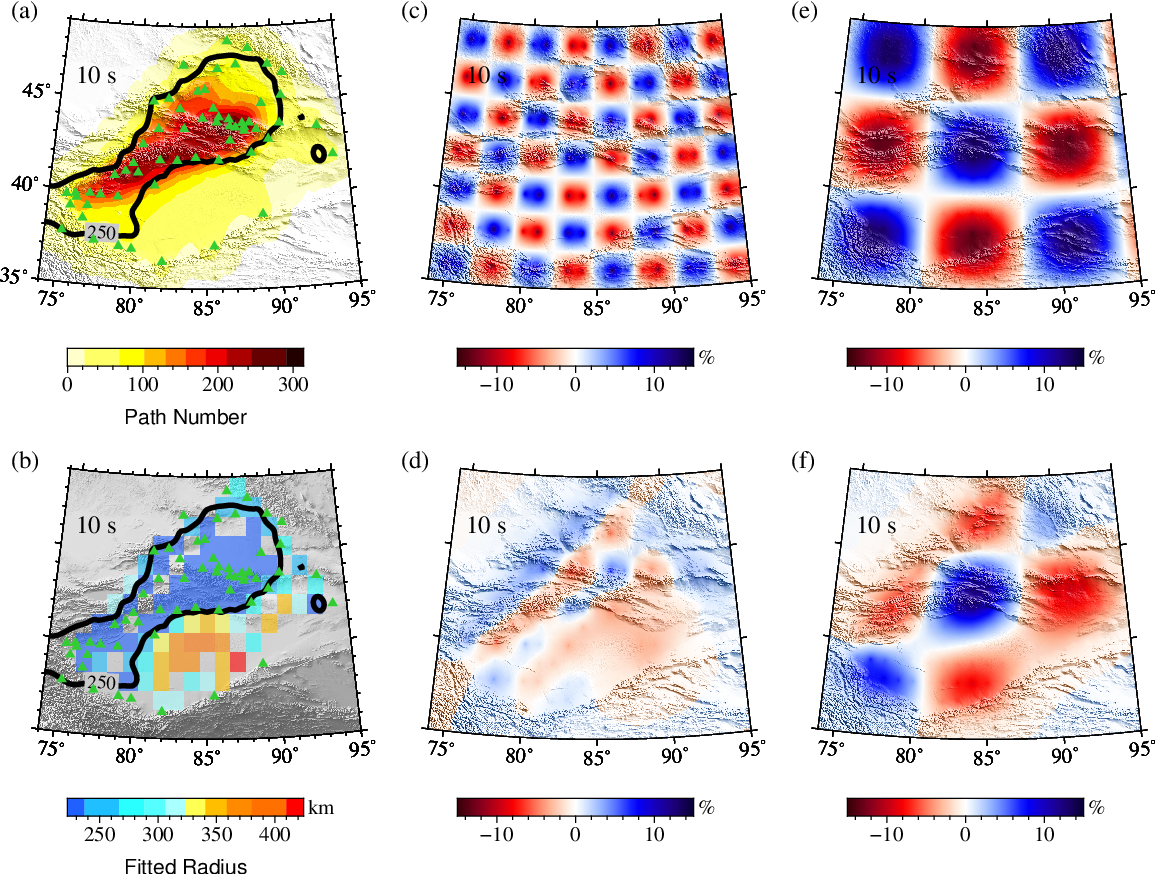
\includegraphics[width=0.75\textwidth]{resolution}
\begin{minipage}{0.9\textwidth}
\footnotesize
\vspace{0.2em}
\textbf{Fig. 3.}
\itshape
Rayleigh group velocity tomography at  10 s. (a) 2D group velocity perturbation
map refers to $2.69315$ km/s, average group velocity of this area and the colorbar
indicates percent. Solid black line encloses area with resolution better than $250$ km/s.
(b) Fitted radius distribution from resolution matrix. Black triangles indicates locations
of seismic stations. Synthetic model (c) for checkerboard test and its recovered one (d).
These models have similar symbols with panel (a).
\end{minipage}
\end{center}

\begin{center}
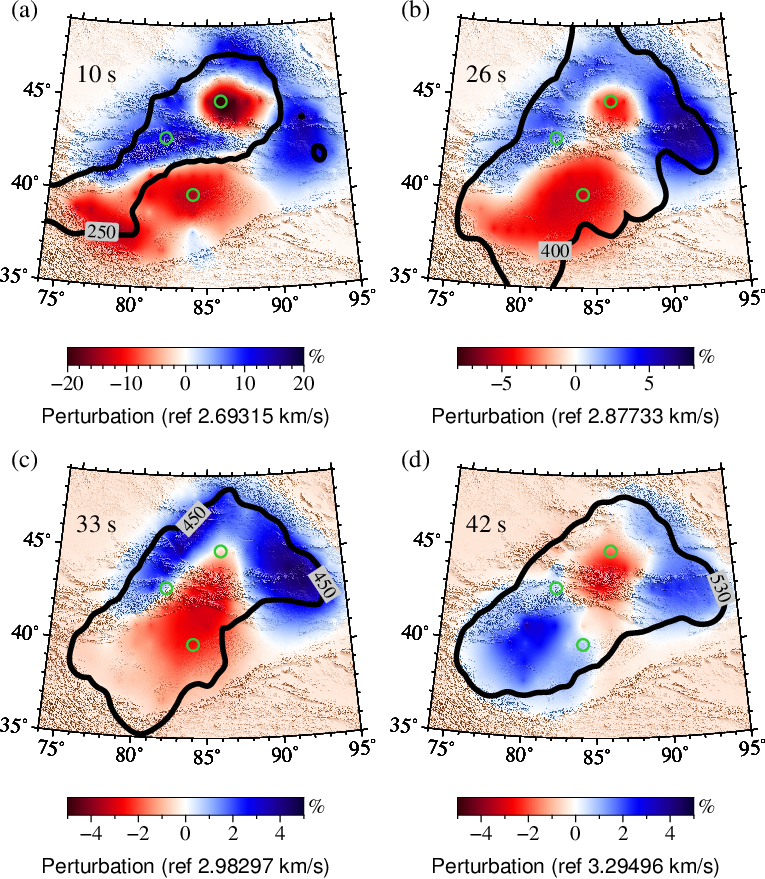
\includegraphics[width=0.75\textwidth]{maps}
\begin{minipage}{0.9\textwidth}
\footnotesize
\vspace{0.2em}
\textbf{Fig. 4.}
\itshape
Rayleigh group velocity perturbation relative to the median velocity at periods
10, 26, 33 and 42 s. The solid black line enclosed main area with resolution than
labeled value. Three circles represent representative points to represent Tarim basin, Tian Shan Mt.
and Junggar basin, separately, at which 1D shear velocity models are inverted in later section.
\end{minipage}
\end{center}

\end{posterbox}

\begin{posterbox}[column=2 ]{4. Shear wave velocity models}
Surface wave tomography result provides Rayleigh group velocity dispersion curves
at any points to do Monte Carlo Markov Chain inversion for three typical geological
part.


\vspace{-0.1cm}
\begin{center}
\begin{tikzpicture}[nodes={inner sep=0}]
\node (a) at (-0.75,-0.2) {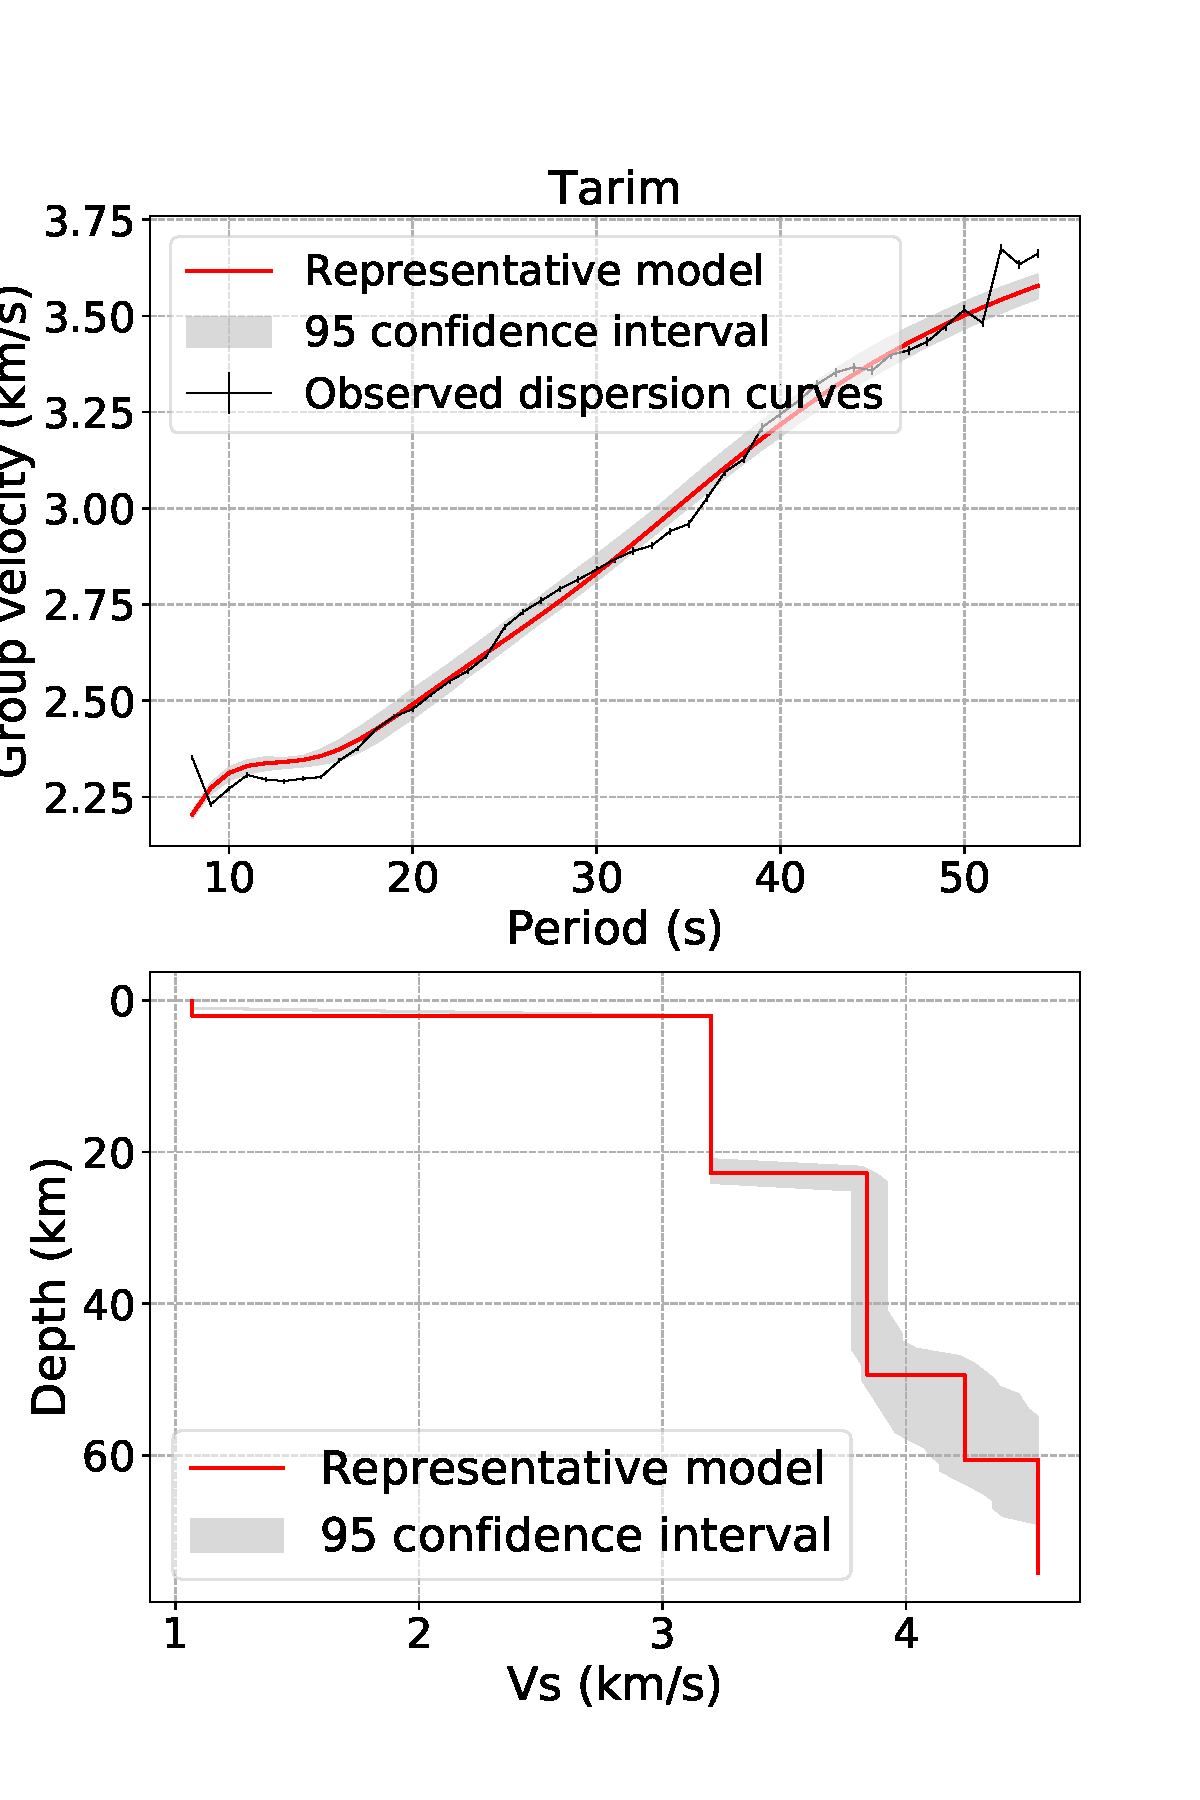
\includegraphics[width=0.33\textwidth]{Tarim}};
\node (b) at (4.2,-0.2) {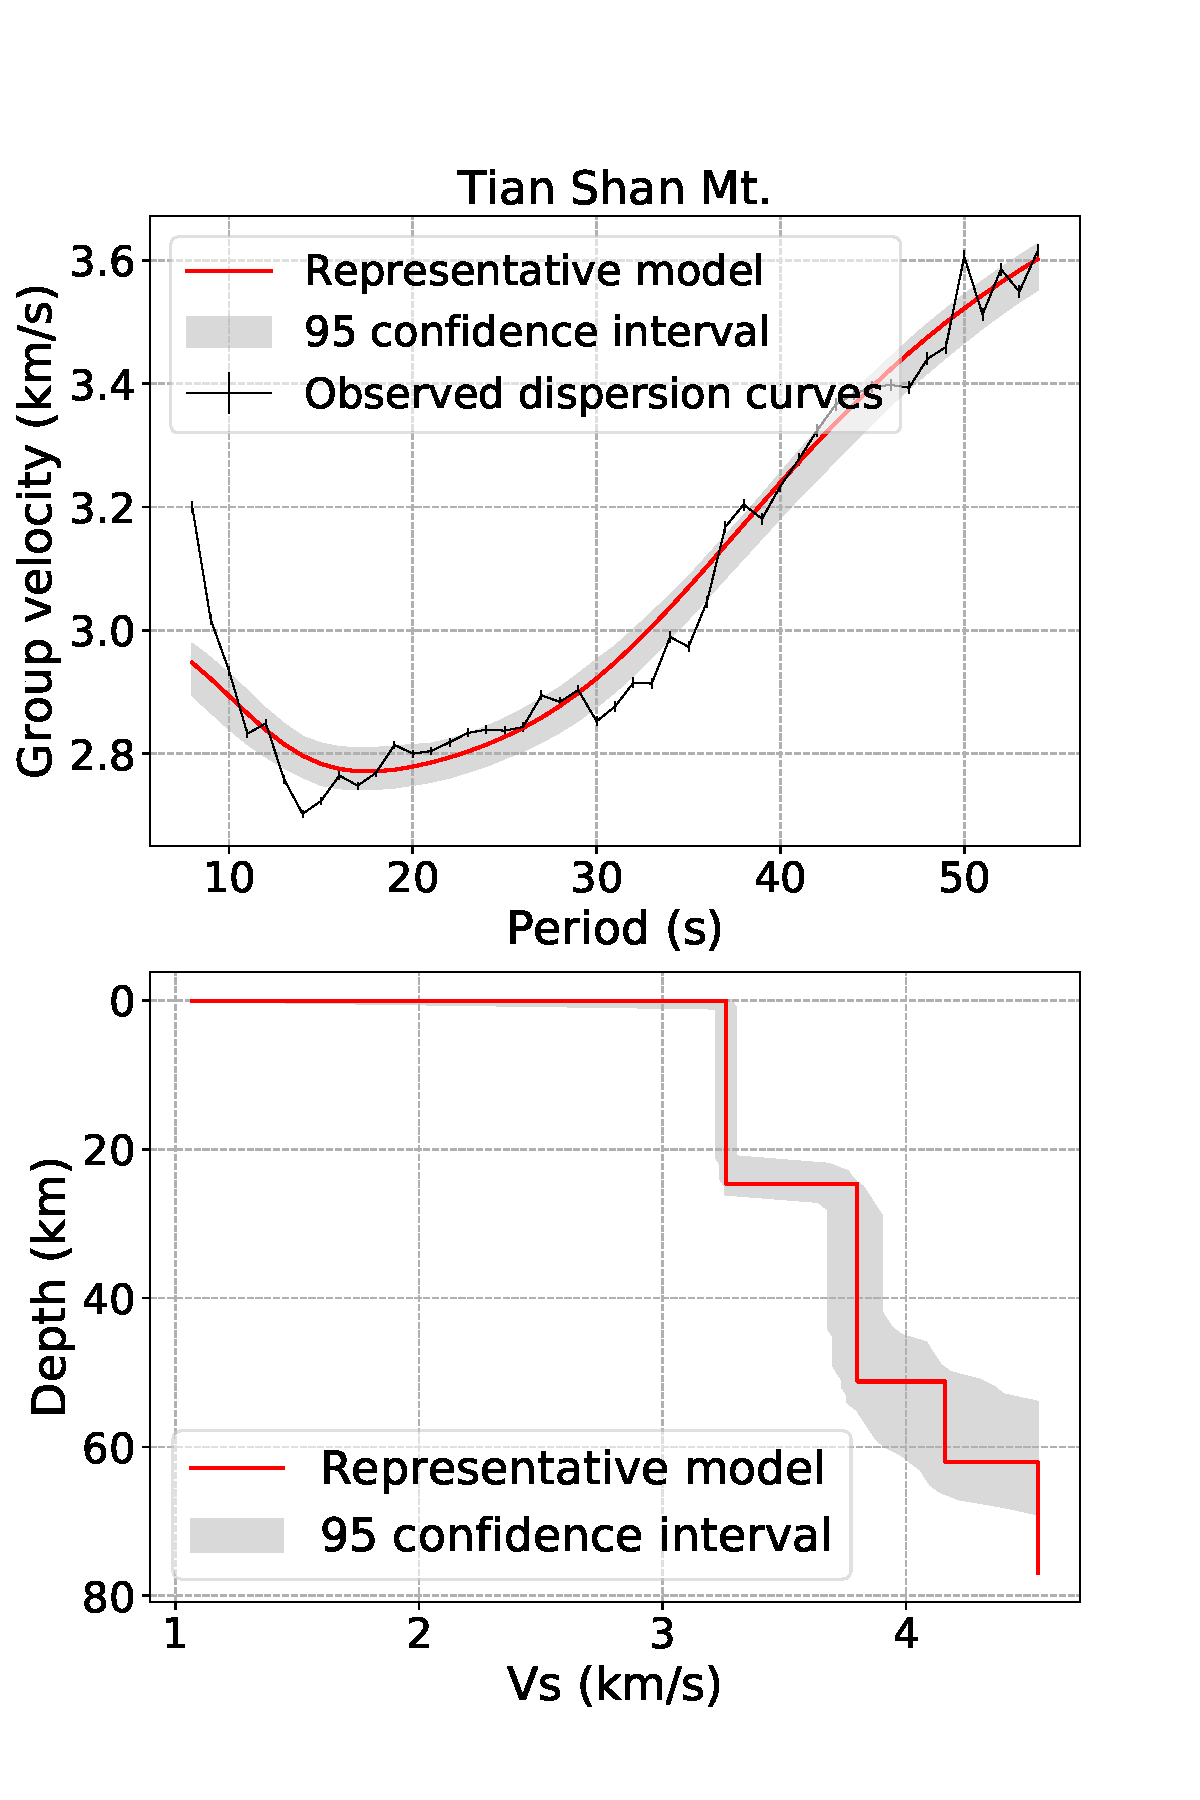
\includegraphics[width=0.33\textwidth]{tianshan}};
\node (c) at (9.0,-0.2) {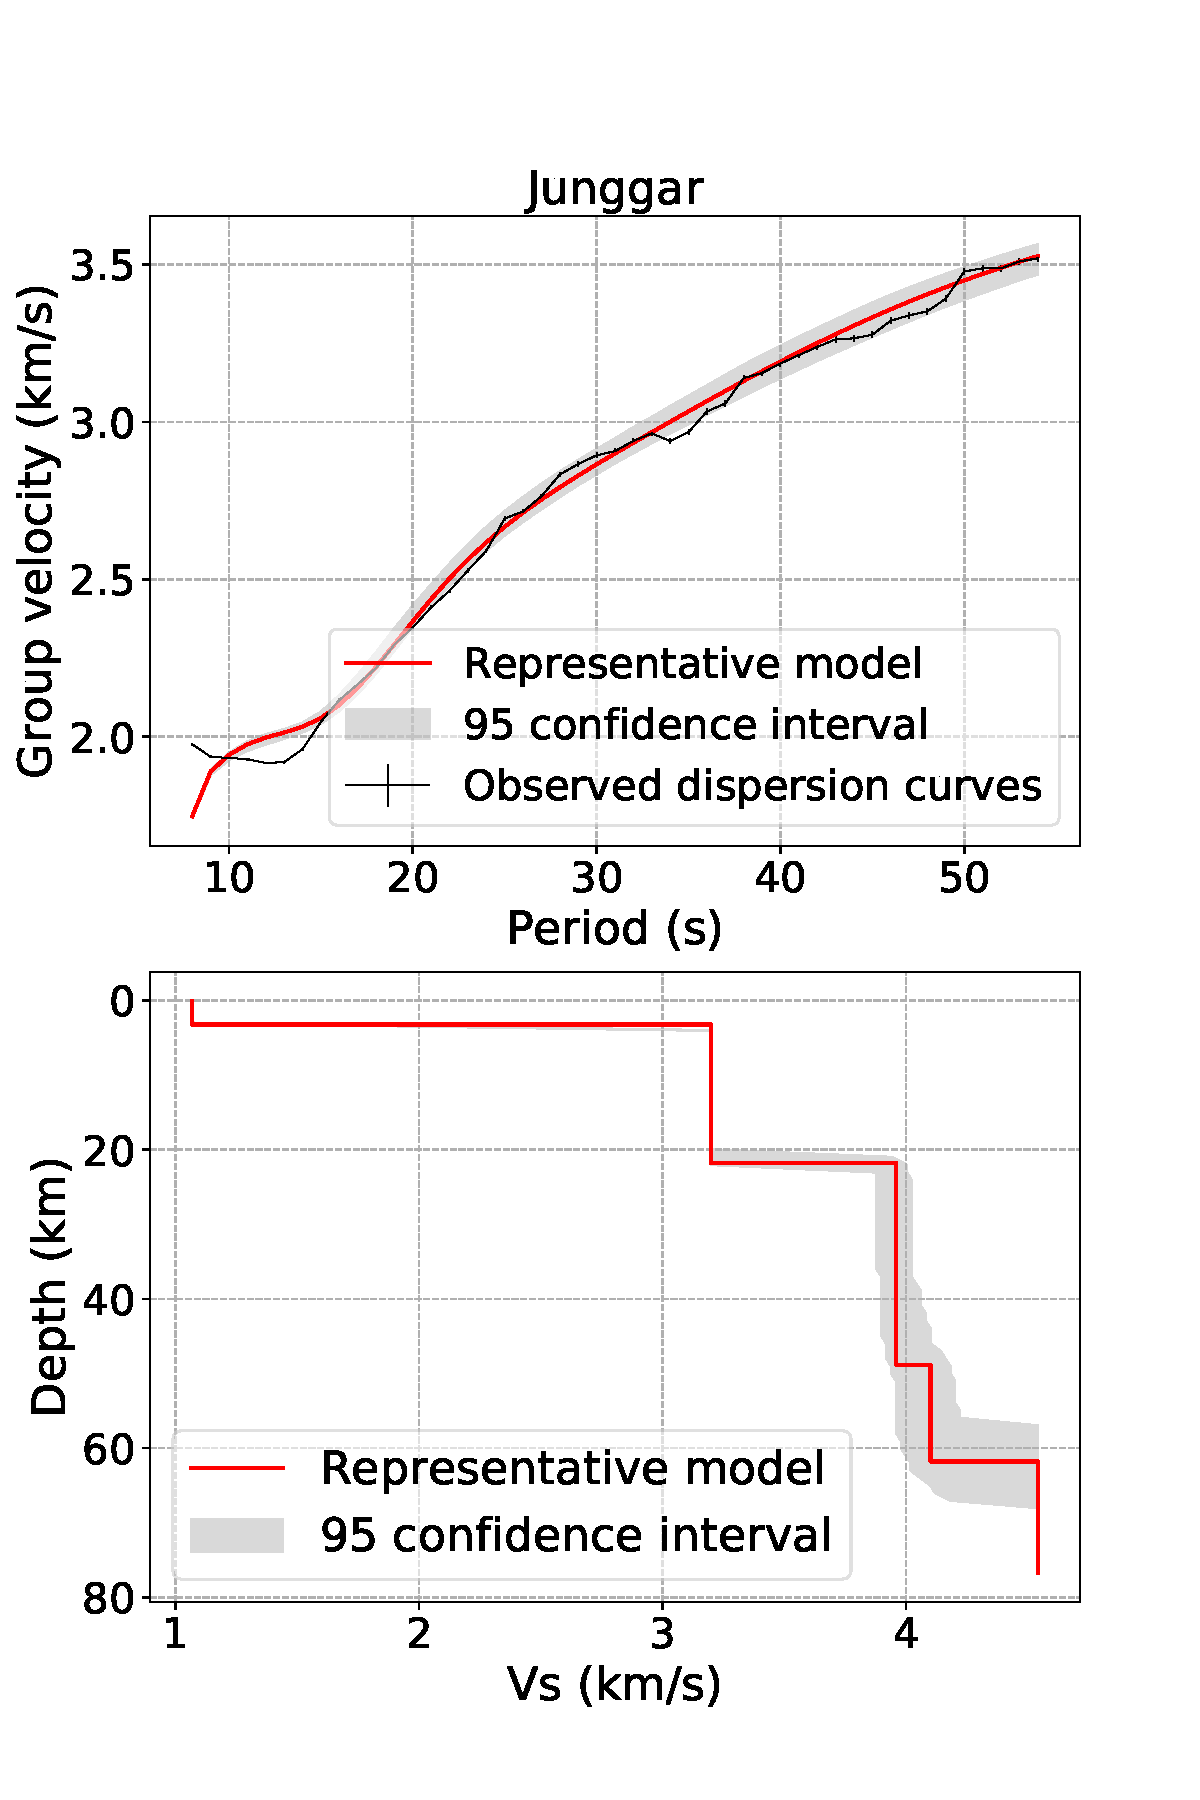
\includegraphics[width=0.33\textwidth]{Junggar}};
\node at (-3.05, 3.2) {(a)};
\node at (1.9, 3.2) {(b)};
\node at (6.7, 3.2) {(c)};
\end{tikzpicture}


\begin{minipage}{0.9\textwidth}
\small
\textbf{Fig. 5.}
\itshape
Inverted models at three representative points, locating at Tarim basin, Tian Shan Mountain and Junggar basin, separately.
Observed dispersion curves (solid black lines with error bars) are extracted from 2D rayleigh group velocity maps.
Shade areas show the 95 percent confidence interval of the shear velocity model (below) and theoretical
group velocity dispersion curve (upper). Red lines represents representative shear velocity model (below)
and its synthetic dispersion curve (upper), which is cloesest to the average of all sampled models.
\end{minipage}
\end{center}



\begin{center}
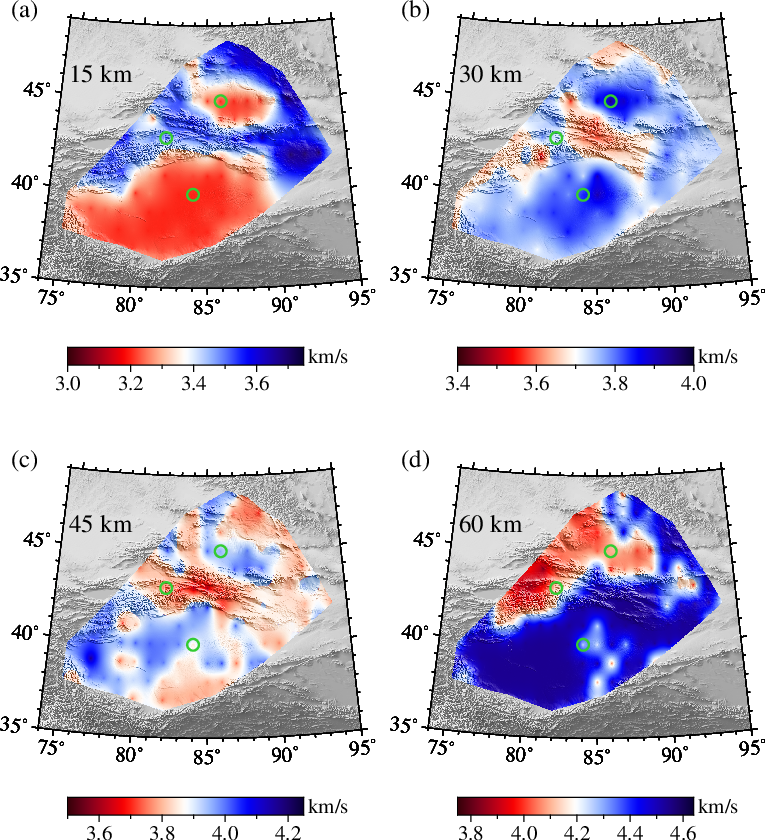
\includegraphics[width=0.75\textwidth]{shear_velocity_maps}
\begin{minipage}{0.9\textwidth}
\footnotesize
\vspace{0.2em}
\textbf{Fig. 6.}
\itshape
 Shear wave velocity maps at depths 15 , 30, 45 and 60 km. Colored area indicates where there is path coverage.
 The green circles show locations of typical 1D shear wave velocity.
\end{minipage}
\end{center}

\end{posterbox}

\begin{posterbox}[column=2, below=auto]{5. Conclusions}
We collect a large dataset of high-quality PKiKP waveforms, and use
PKiKP-PcP differential travel time residuals, PKiKP/PcP amplitude ratios,
and PKiKP-PcP waveform differences to constrain ICB properties.
Based on the observations, the ICB beneath Bearing Sea has a sharp and flat
boundary, and the ICB beneath Mexico may have a bumpy ICB with a topographic
height change of 5 km. PKiKP/PcP amplitude ratios are much larger than predictions,
implying possible other factors which affects the amplitude ratios.
\end{posterbox}

\end{poster}
\end{document}
